\documentclass[a4paper,12pt]{article}
\usepackage{graphicx}
\usepackage[a4paper, total={6in, 9in}]{geometry}
\usepackage[T1]{fontenc}
\usepackage[utf8]{inputenc}
\usepackage{graphicx}
\usepackage{tikz}
\usepackage{float}
\usepackage{mathtools}
\usepackage{fancyhdr}
\usepackage{caption}
\usepackage{textgreek}
\usepackage{yfonts}
\graphicspath{/home/Desktop/IST/2ano/1semestre/2quarter/SS/relatorio/}
\renewcommand{\figurename}{Figura}
\renewcommand{\contentsname}{Índice}
\renewcommand{\refname}{Bibliografia}
\pagestyle{fancy}
\date{Janeiro-Fevereiro 2022}
\title{Sinais e Sistemas \\ \large {Relatório Laboratorial}}
\author{
\\ João Barreiros C. Rodrigues nº99968
\\Vasco Maria  Aguiar M. R. Esteves nº 100110 }

\begin{document}
	\pagenumbering{gobble}
	\begin{titlepage} % Suppresses displaying the page number on the title page and the subsequent page counts as page 1
        \newcommand{\HRule}{\rule{\linewidth}{0.5mm}} % Defines a new command for horizontal lines, change thickness here
        \center % Centre everything on the page
        \textsc{\LARGE Instituto Superior Técnico}\\[1.5cm] % Main heading such as the name of your university/college
	\textsc{\Large Licenciatura em Engenharia Eletrotécnica e de Computadores}\\[0.25cm]
        \textsc{\Large Sinais e Sistemas}\\[0.5cm] % Major heading such as course name
        \HRule\\[0.4cm]
        {\huge\bfseries Relatório Laboratorial}\\[0.4cm] % Title of your document
        \HRule\\[1.5cm]\
        João \textsc{Barreiros C. Rodrigues} nº99968 , LEEC\\
	Vasco Maria \textsc{Aguiar M. R. Esteves} nº 100110, LEEC
        \vfill\vfill\vfill % Position the date 3/4 down the remaining page
        {\large Janeiro-Fevereiro 2022} % Date, change the \today to a set date if you want to be precise
        \vfill % Push the date up 1/4 of the remaining page
\end{titlepage}
	\pagenumbering{arabic}
	\newpage
		\tableofcontents
	\newpage
	\section{Análise de um sistema (R1-R5)}
		\subsection{Questão R1}
			\paragraph{Da definição algébrica de \textit{linearidade} compreende-se que um sistema linear deve obedecer às condições seguintes:}
				\subparagraph{\textbf{Aditividade:} Verifica-se que: \textit{sistema(x+y)=sistema(x)+sistema(y)}}
				\subparagraph{\textbf{Homogeneidade: Verifica-se que: \textit{sistema(}}\textbf{\alpha \textit{y)=} \alpha \textbf{\textit{sistema(y)}}}} \mbox{}\\ \mbox{}\\
			É possível testar a primeira condição executando:
			\begin{figure}[H]
				\centering
					\captionsetup{justification=centering}
					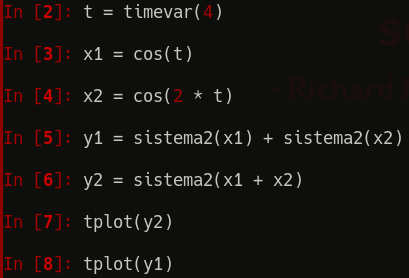
\includegraphics[width=0.5\textwidth]{r1code01.png}
					\caption{Síntese de dois sinais x1 e x2 e síntese de dois sinais y1 e y2 por respectiva soma dos outputs da passagem individual de x1   e x2 pelo sistema 1 e pela passagem do sinal resultante da soma de x1 com x2 pelo sistema1.}
			\end{figure}
			Para o qual se obtém o output:
			\begin{figure}[H]
  				\centering
  				\captionsetup{justification=centering}
  				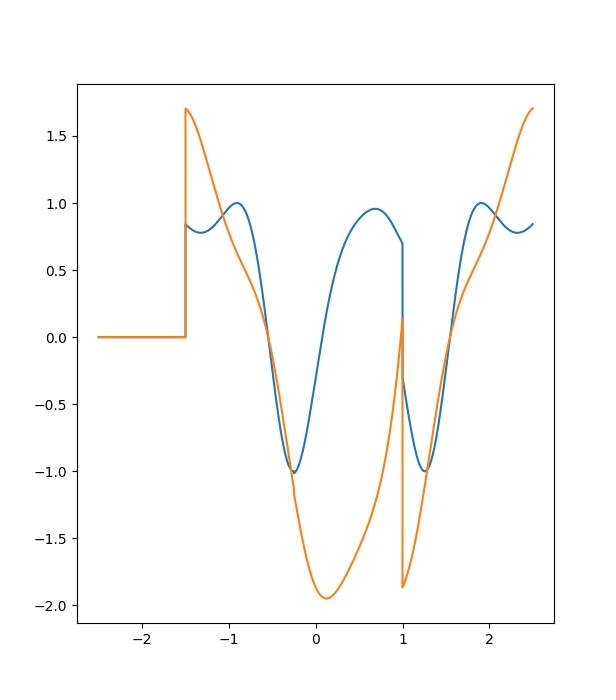
\includegraphics[scale=0.35\textscale]  {r1graph01.png}
				\caption{A azul e a laranja, respectivamente as representações gráficas de y1 e y2, de notar que y1 \neq y2.}
			\end{figure}
			Verificando assim que o sistema não é aditivo, precipitando para a conclusão da  \textbf{não-linearidade do sistema.}\\
			Embora a linearidade seja uma conjunção de duas propriedades, realiza-se também o teste da condição de homogeneidade para efeitos de estudo:
 			\begin{figure}[H]
  				\centering
  				\captionsetup{justification=centering}
  				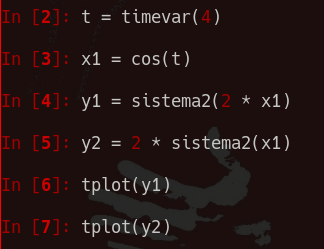
\includegraphics[width=0.3\textwidth]{r1code02.png}
				\caption{Síntese de um sinal x1 e síntese de dois sinais y1 e y2 por respectiva passagem do produto de x1 com uma contante \textbeta (tal que \textbeta =2) pelo sistema 2 e pelo produto do resultado da passagem de x1 pelo sistema 2 com \textbeta.}
  			\end{figure}
			Para o qual se obtém os outputs:
			\begin{figure}[H]
    				\centering
    				\captionsetup{justification=centering}
    				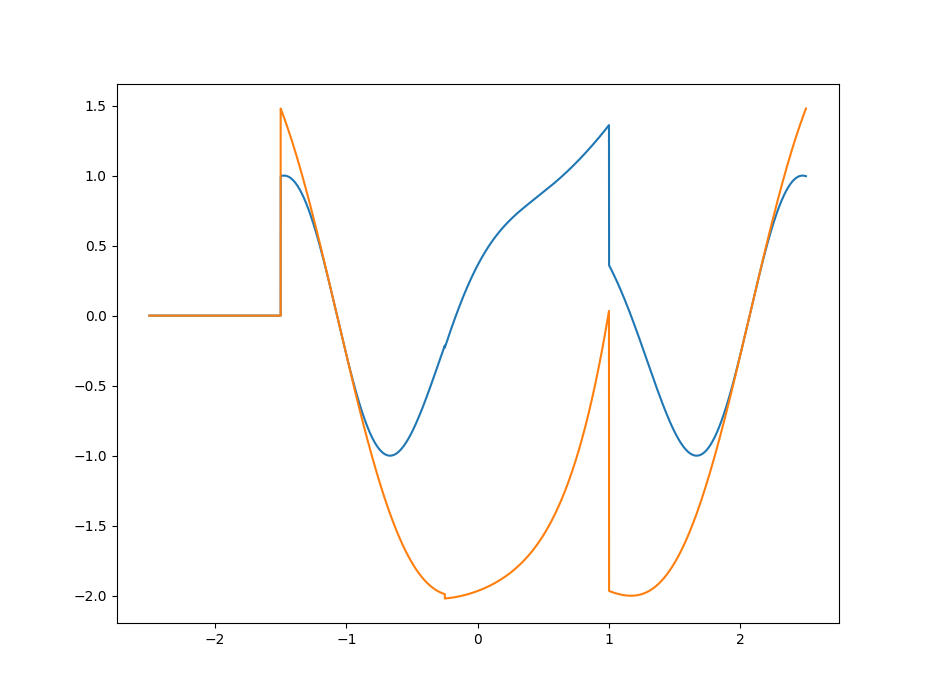
\includegraphics[scale=0.4\textscale]  {r1graph02.png}
				\caption{A azul e a laranja, respectivamente as representações gráficas de y1   e y2, de notar que y1 \neq y2.}
  			\end{figure}
			Provando adicionalmente que o sistema \textbf{não é homogéneo}
			\newpage

		\subsection{Questão R2}
			\paragraph{Definem-se sistemas invariantes no tempo aqueles que não dependem directamente da variável tempo, ou seja na expressão matemática do sistema não está comtemplada a variável tempo. O sistema invariante no tempo pode contudo depender indirectamente do tempo, ou seja a função de \textit{input} dada pode depender explicitamente do tempo.}
			\mbox{}\\
			\mbox{}\\
			Desta forma, o mais simples teste que se pode realizar de forma a concluir a variância ou invariância no tempo de um sistema é através do deslocamento do sinal de entrada.
			O sistema será invariante no tempo se a seguinte proposição for verdadeira:
			\mbox{}\\
			\mbox{} \\
			\mbox{		} \textit{Para x$_0$(t) e x$_1$(t)=x$_0$(t+\textbeta) ou seja x$_1$(t)= \mathbb{T}$_\beta$ x$_0$(t)
			\\ 
			\mbox{          } \mathbb{T}$_\beta$ sistema(x$_0$)=sistema(x$_1$)}
			\mbox{}\\
			\mbox{          } Considerando \mathbb{T}$_\beta$ o operador deslocamento para o vector (0,-\textbeta)
\mbox{}\\\mbox{}\\
			Tomando as noções anteriores computa-se no ambiente \textit{ipython}:
			\begin{figure}[H]
    				\centering
    				\captionsetup{justification=centering}
    				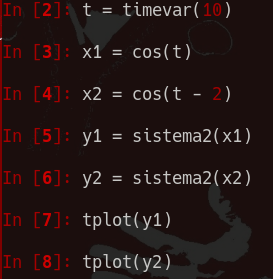
\includegraphics[width=0.3\textwidth]{r2code01.png}
				\caption{Síntese de um sinal x1 e  x2, tal que x2=\mathbb{T} $_-$$_2$ e síntese de dois sinais y1 e y2 por respectiva passagem de x1 e x2 pelo sistema2.}
    			\end{figure}
			Para o qual se obtém os outputs:
 			\begin{figure}[H]
      				\centering
      				\captionsetup{justification=centering}
      				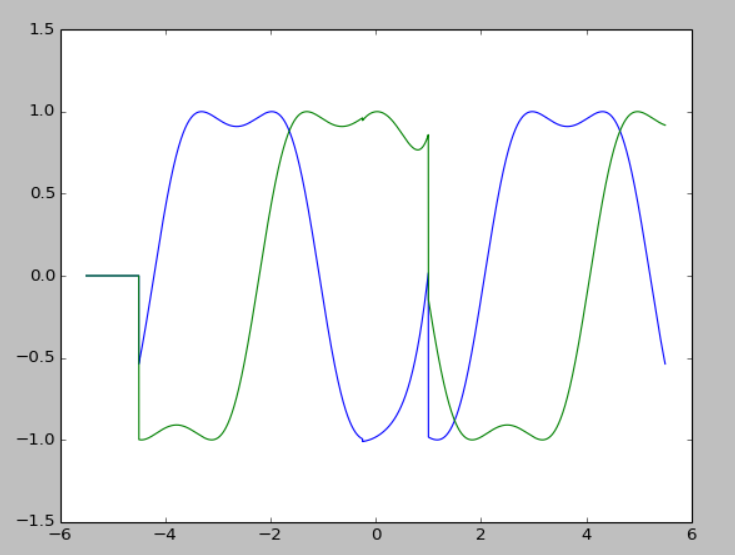
\includegraphics[scale=0.3\textscale]{r2graph.png}
				\caption{A azul e a verde, respectivamente, os sinais y1 e y2. De notar a distinção entre a forma de onda de y1 e y2, indiciando que \mathbb{T} $_-$$_2$ y1\neq y2.}
      			\end{figure}
			Concluindo-se que o sistema 2 \textbf{não é invariante no tempo}
	\newpage	
		\subsection{Questão R3}
			\paragraph{Sucintamente, um sistema descreve-se como sem memória se o seu output para um instante t$_1$ for dependente apenas do input dado nesse mesmo instante.}
			\mbox{}\\
			\mbox{}\\
			Desta forma é possível aferir que um sistema sem memória tem todas as suas referências canônicas à variável tempo em \textit{input}(t) na forma:
			\\ 
			\begin{center}
				\textalpha $t^{\gamma}$ +\textbeta , com \textalpha = 1, \textgamma=1 e \textbeta=0.
			\end{center}
			Um teste simples que pode ser utilizado para verificar esta propriedade consiste na síntese de dois sinais x$_0$ e x$_1$ distintos que se intersetam em determinado instante t$_i$. Para um sistema de equação y$_1$ o sistema será sem memória se y$_1$(x$_0$) e y$_1$(x$_1$) se intersetarem em t$_i$.
			\mbox{}\\
			\mbox{}\\
			Executando o referido teste:
			\begin{figure}[H]
      				\centering
      				\captionsetup{justification=centering}
      				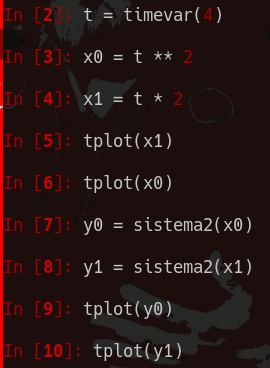
\includegraphics[width=0.2\textwidth]{r3code01.png}
				\caption{Realização em ambiente \textit{ipython} do teste acima descrito.}
      			\end{figure}
			Do qual se obtém o primeiro \textit{output}, de controlo:
			\begin{figure}[H]
        			\centering
        			\captionsetup{justification=centering}
        			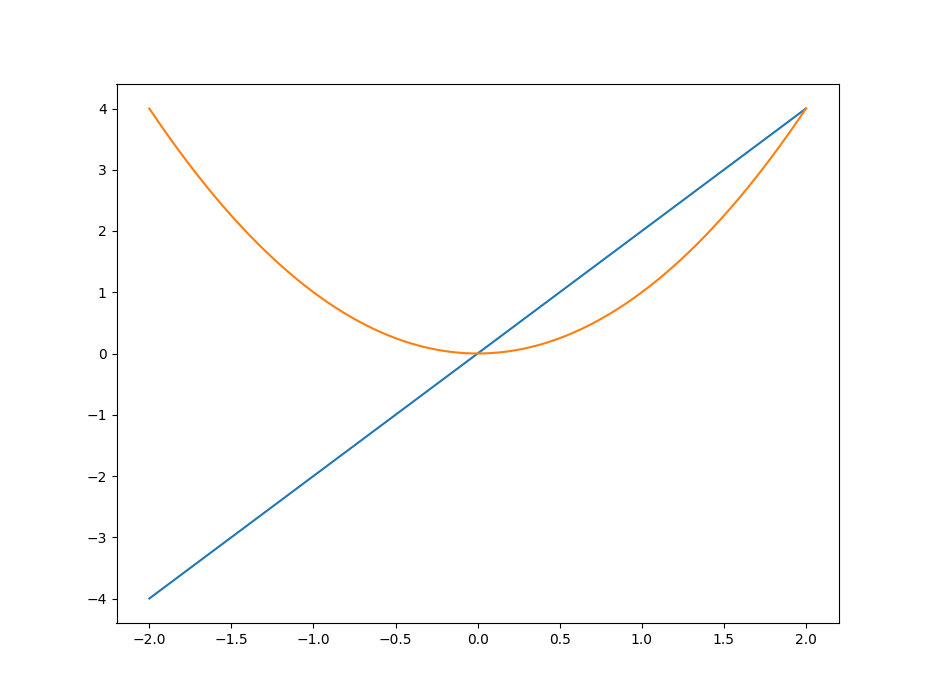
\includegraphics[scale=0.35\textscale]{r3graph01.png}
				\caption{Representação gráfica de x1 (a azul) e x0 (a laranja). De notar a intersecção dos gráficos para t=0 e t=2.}
        		\end{figure}
			E o segundo, conclusivo:
			\begin{figure}[H]
       	 			\centering
        			\captionsetup{justification=centering}
        			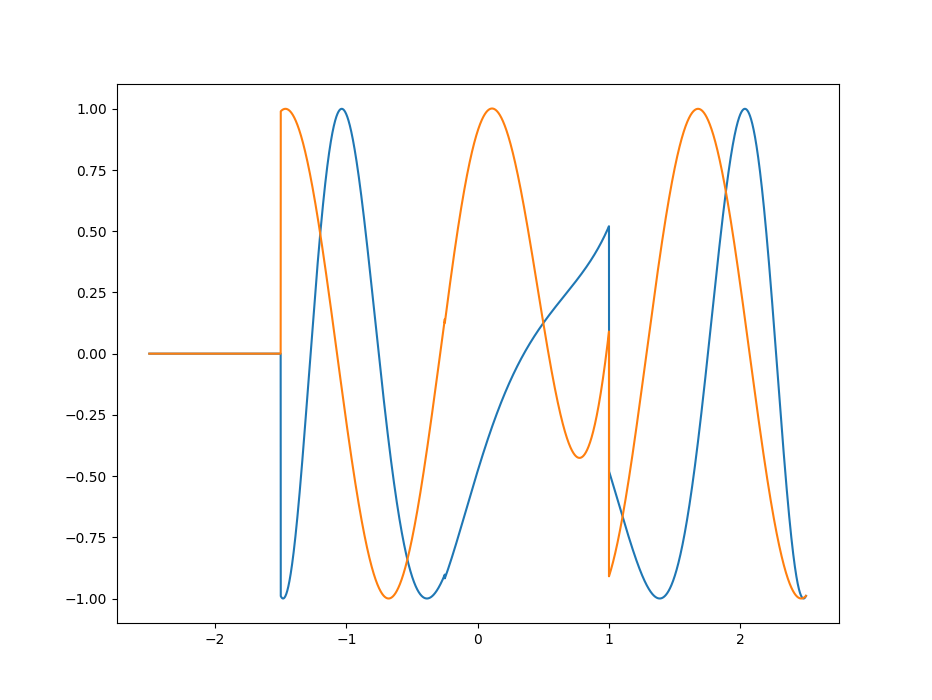
\includegraphics[scale=0.35\textscale]{r3graph02.png}
				\caption{Representação gráfica de y0 (a azul) e y1 (a laranja). Verifique-se a não intersecção do gráficos em t=0 e t=2.}
			\end{figure}
			Prova-se que o sistema 2 \textbf{tem memória}.
		\newpage
		\subsection{Questão R4}
			\paragraph{Assim como na caracterização da memória do sistema, também a definição de causalidade assenta nas particularidades do sistema relativas à variável tempo. Desta forma um sistema descreve-se como causal quando o  seu output para qualquer instante t$_1$ for dependente apenas de inputs presentes ou passados ou seja t$_1$ \ge t _{input}}\mbox{  }\\ \mbox{}\\
			Desta forma é possível aferir que um sistema causal tem todas as suas referências canônicas à variável tempo em \textit{input}(t) na forma:\\
			\begin{center} 
				\begin{math}
					\alpha t^{\gamma}$ +\beta , com \alpha \in ]0,1[, \gamma \in ]0,  1] \mbox{  }e \mbox{  }\beta  \in ]- \infty , 0]. 
				\end{math}
			\end{center}
			Desta forma, para determinar um possível contra-exemplo utilizam-se sinais de tipo \textit{degrau} (nos testes apresentados utilizam-se degrau unitário, linear, sinusoidal e exponencial) tal que para t < 0 x$_n$ é igual a 0. Assim caso o sinal de saída $sistema(x$_t$(t)) \neq 0$ para t < 0 compreende-se o adiantamento do sinal ou seja o output está a depender de inputs futuros, ou seja viola-se a definição inicialmente estipulada para a causalidade.
			\newpage
			Assim computa-se o setup inicial:
			\begin{figure}[H]
                        	\centering
                        	\captionsetup{justification=centering}
                        	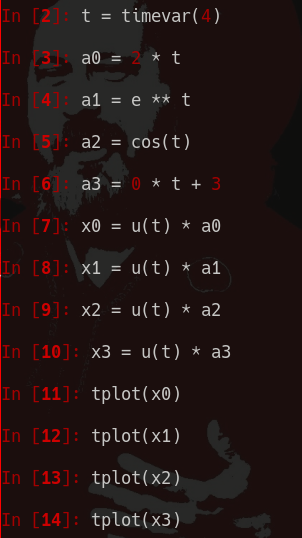
\includegraphics[width=0.3\textwidth]{r4code01.png}
	        		\caption{Síntese dos sinais acima propostos, com degrau linear x0, degrau exponencial x1, degrau sinusoidal x2 e degrau unitário x3.}
                	\end{figure}
			Para o qual se obtém o output:
			\begin{figure}[H]
                        	\centering
                        	\captionsetup{justification=centering}
                        	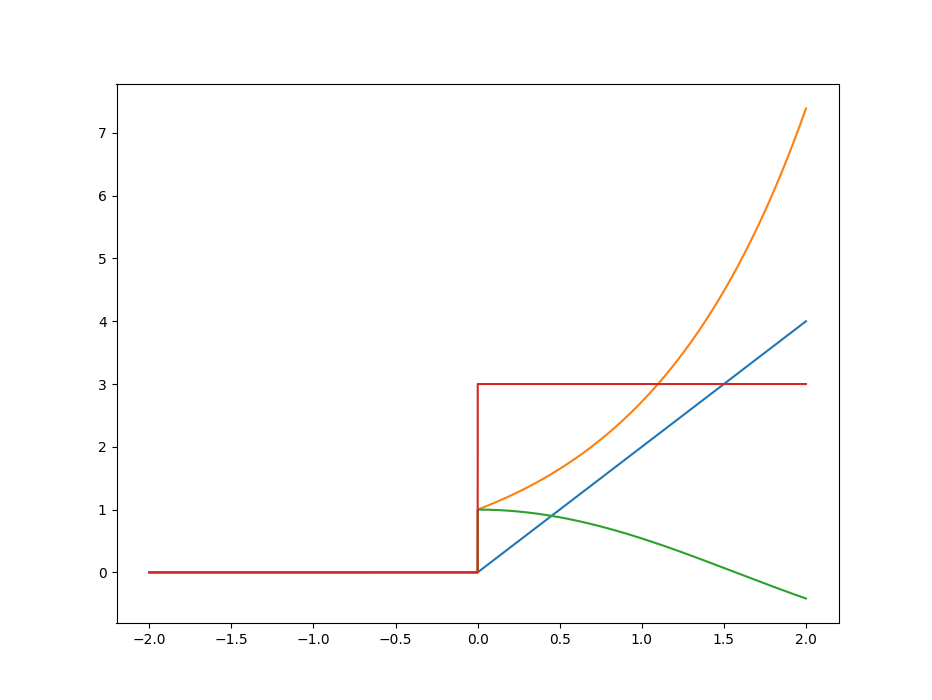
\includegraphics[scale=0.35\textscale]{r4graph01.png}
                		\caption{Representação gráfica dos sinais de input sintetizados. A azul, laranja, verde e vermelho respectivamente x0, x1, x2 e x3.}
                	\end{figure}
			\newpage
			De seguida computa-se o setup secundário:
			\begin{figure}[H]
	        		\centering
        	        	\captionsetup{justification=centering}
                		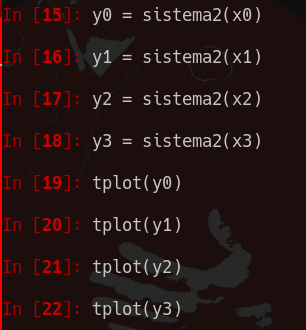
\includegraphics[width=0.3\textwidth]{r4code02.png}
                        	\caption{Síntese dos sinais de output y$_n$.}
                	\end{figure}
			Para o qual se obtém o output:
			\begin{figure}[H]
                        	\centering
                          	\captionsetup{justification=centering}
                          	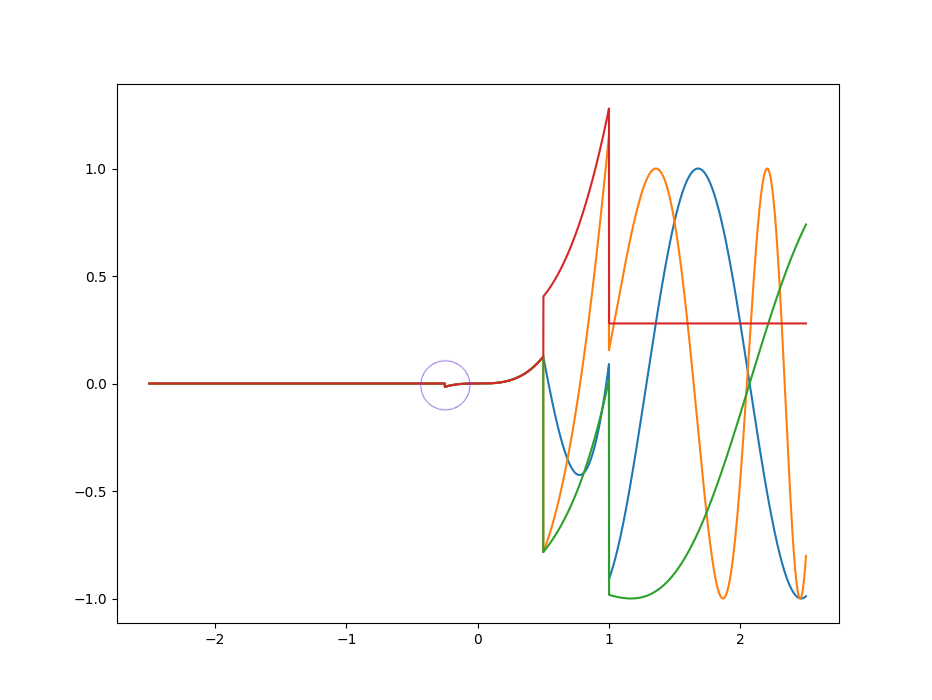
\includegraphics[scale=0.4\textscale]{r4graph02.1.png}
                          	\caption{Representação gráfica dos sinais de output, com sinal coincidente ao input respectivo. Adicionalmente não se considera a oscilação do sinal circundada a roxo, proveniente das limitações do ambiente em que as experiências foram realizadas.}
                  	\end{figure}
			Verifica-se que para os sinais dados (propositalmente de equações distintas) a condição inicial que sustenta a definição de causalidade não é quebrada uma vez que nenhum dos sinais y$_n$ possui para t<0 valor $\neq 0$ ou seja não é presente nenhuma evidência que o sistema2 provoque o adiantamento do sinal.\\ \mbox{} \\
		Mantém-se então a hipótese que o sistema \textbf{possa ser causal}.
		\newpage
		\subsection{Questão R5}
			\paragraph{Sucintamente define-se um sistema estável como um sistema que para um input com pequenas oscilações não diverge}\mbox{}\\\mbox{}\\
			Um teste válido para determinar um contra-exemplo para a estabilidade de um sistema é a utilização de inputs limitados superior e inferiormente (nos testes apresentados utilizam-se degrau unitário e sinal sinusoidal). Desta forma caso o sinal de output pelo sistema sintetizado divergir prova-se que o sistema não é estável.\\
			Assim em ambiente \textit{ipython} computa-se:
                  	\begin{figure}[H]
                        	\centering
                        	\captionsetup{justification=centering}
                        	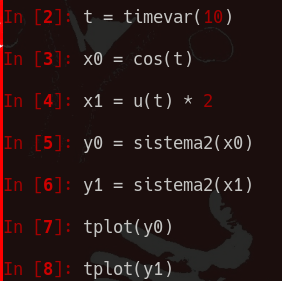
\includegraphics[width=0.3\textwidth]{r5code01.png}
                		\caption{Síntese dos sinais x0 e x1, demonstrados em alíneas anteriores como sendo limitados. Síntese dos sinais de output y$_n$ pela passagem dos respectivos sinais x$_n$ pelo sistema 2.}
                  		\end{figure}
                	Para o qual se obtém o output gráfico:
                  	\begin{figure}[H]
                        	\centering
                        	\captionsetup{justification=centering}
                		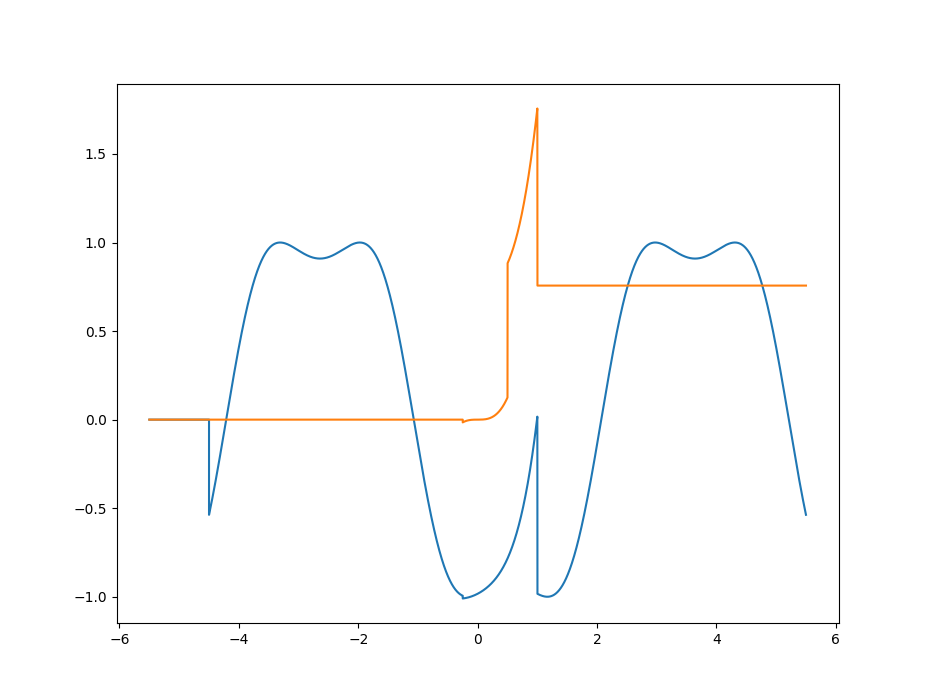
\includegraphics[scale=0.4\textscale]{r5graph01.png}
                		\caption{Representação gráfica dos sinais de output. De notar que ambos os sinais de output são limitados superior e inferiormente.}
			\end{figure}
			Desta forma não foi possível sintetizar um contra-exemplo mantendo-se a hipótese da \textbf{possível estabilidade do sistema}.
	\section{Filtragem (R6-R9)}
		\subsection{Questão R6}
			\paragraph{Da expressão deduzida de |H(j$\omega$)|:} \mbox{}\\ \mbox{} \\
			\begin{center}
				H(j$\omega$)= $\frac{1}{1+j\omega RC}$ $\iff$ \\ \mbox{}\\
				|H(j$\omega$)|= $\frac{1}{\sqrt{(1+j\omega RC)^{2}}}$ $\iff$\\ \mbox{}\\
				R= $\frac{\sqrt{\frac{1}{|H(j\omega)|^{2}}-1}}{\omega C}$
			\end{center}
			Obtém-se os valores de |H(j$\omega$)| pela computação no sistema \textit{ipython}:
			\begin{figure}[H]
                        	\centering
                                \captionsetup{justification=centering}
                        	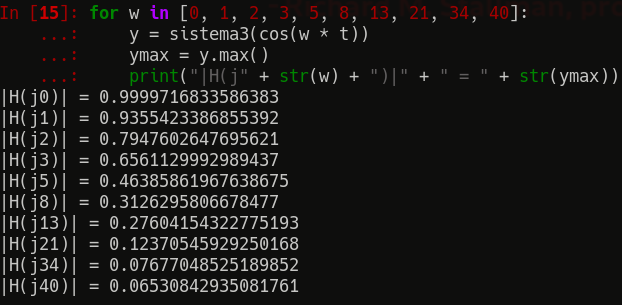
\includegraphics[width=0.7\textwidth]{r6code01.png}
				\caption{Determinação de |H(j$\omega$)| para vários $\omega$.}
          			\end{figure}
			  Calculando R pela relação anteriormente estabelecida e cruzamento de dados:\\
			\begin{center}
			  \begin{tabular}{||l|c|r||}
			    	\cline{1-3}
    					$\omega$ & |H(j$\omega$)| & R /$\Omega$  \\
    				\hline \hline
    					1 & 0.93554 &  755.12 \\
    				\hline
    					2 & 0.79476 & 763.66 \\
    				\hline
    					3 & 0.65611 & 766.81 \\
				\hline
                                	5 & 0.46385 &  763.96 \\
				\hline
                                	8 & 0.31262 & 759.61\\
				\hline
                                	21 & 0.12370 & 764 \\
				\hline
                                	34 & 0.076770 & 763.97  \\
				\hline
                                	40 & 0.076770 & 764.06 \\
				\cline{1-3}
			\end{tabular}
		       \end{center}
			Assim R$_m$$_e$$_d$$_i$$_o$ =762.65 $\Omega$.
			\newpage
			Verifica-se a validade do valor médio obtido para R comparando, por exemplo, a representação gráfica do output do sistema 3 com o impulso unitário como input (controlo) e a representação gráfica da expressão:\\
			\begin{center}
				\begin{math}
					h_{C}(t)={\frac {1}{RC}}e^{-{\frac {t}{RC}}}u(t),
				\end{math}
			\end{center}
			Descritiva da resposta de um circuito RC para o impulso unitário, substituindo R por R$_m$$_e$$_d$$_i$$_o$ e C por 500$\mu$F.
			Obtém-se a comparação gráfica no sistema \textit{ipython}:
			\begin{figure}[H]
                                    \centering
                                    \captionsetup{justification=centering}
                                  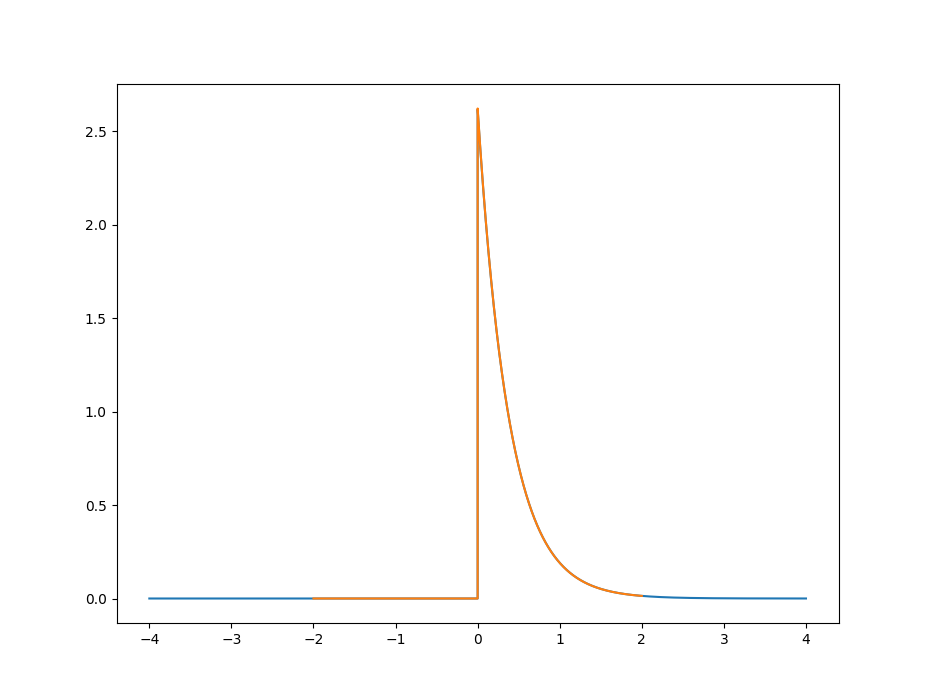
\includegraphics[scale=0.5\textscale]{r6graph01.png}
                                  \caption{A azul o sinal de controlo e a laranja o sinal sintetizado pela substituição das variáveis R e C na equação de resposta do circuito RC. De notar a sobreposição dos dois gráficos, permitindo inferir que o R$_m$$_e$$_d$$_i$$_o$ determinado é solução aproximada de R para o sistema dado.}                        \end{figure}
		\newpage
		\subsection{Questão R7}
			\paragraph{Toma-se como noção inicial que quanto mais rápida for a variação instantânea de um dado sinal x$_n$ em t$_0$ maior será a frequência instantânea nesse mesmo instante no espectro do sinal, \math{F}$_n$.} \mbox{} \\ \mbox{} \\
			\mbox{	}Têm-se então o sinal \textit{p} e o módulo do seu espectro y$_p$, que se utilizarão como controlo dos testes seguintes:
			  \begin{figure}[H]
                                  \centering
                                  \captionsetup{justification=centering}
                                  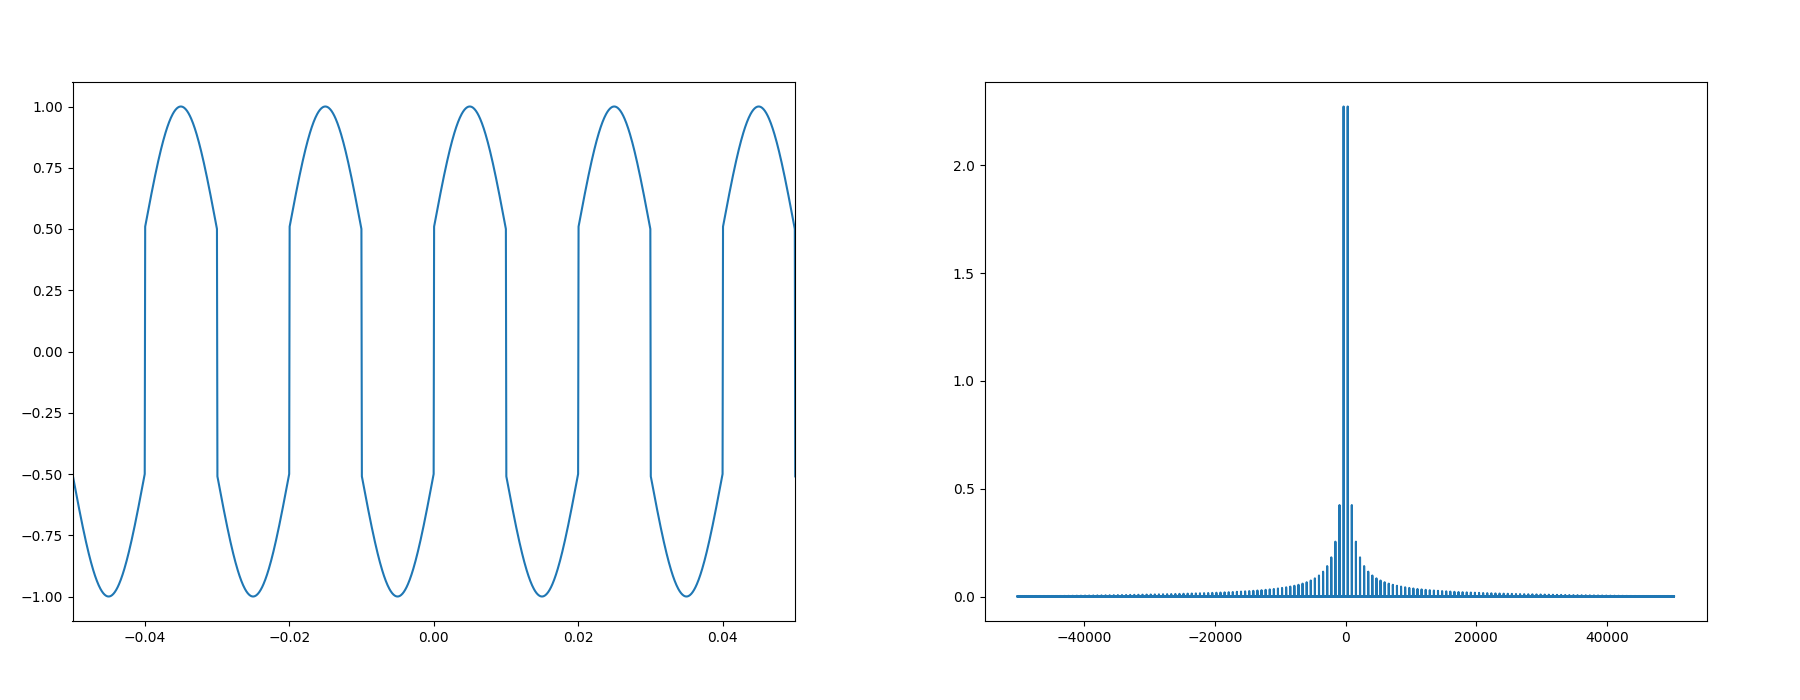
\includegraphics[scale=0.35\textscale]{r7graph01.png}
                                \caption{Representação gráfica do sinal \textit{p} e do módulo do espectro de frequências do sinal \textit{p}, |\math{F}$_p$|}
                          \end{figure}
			Passando \textit{p} pelo sistema 4, identificado como um filtro passa-baixo, e extraíndo o espectro do output:
			  \begin{figure}[H]
                                  \centering
                                  \captionsetup{justification=centering}
                                  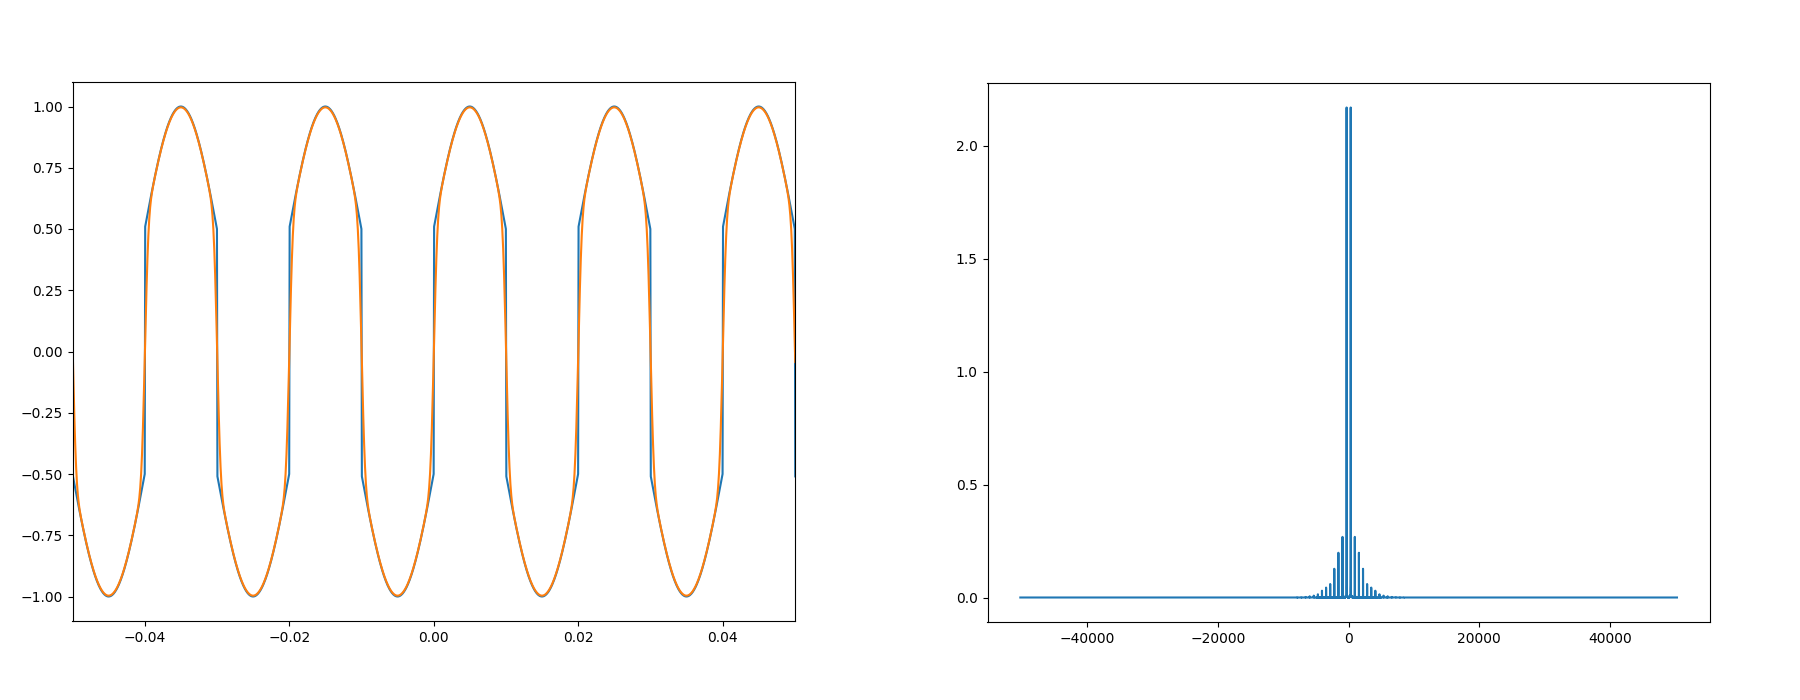
\includegraphics[scale=0.35\textscale]{r7graph02.png}
                                \caption{Representação gráfica do sinal filtrado pelo sistema 4, a laranja (sobreposto sobre o sinal original, a azul) e espectro do sinal filtrado. De notar a distinção nas variações rápidas do sinal, assim como a supressão da frequências mais altas.}
                          \end{figure}
			Logo assim como seria previsível as frequências mais altas são suprimidas, resultando numa pior reprodução das variações rápidas do sinal.
			Passando \textit{p} pelo sistema 5, identificado como um filtro passa-alto, e extraíndo o espectro do output:
                          \begin{figure}[H]
                                  \centering
                                  \captionsetup{justification=centering}
                                  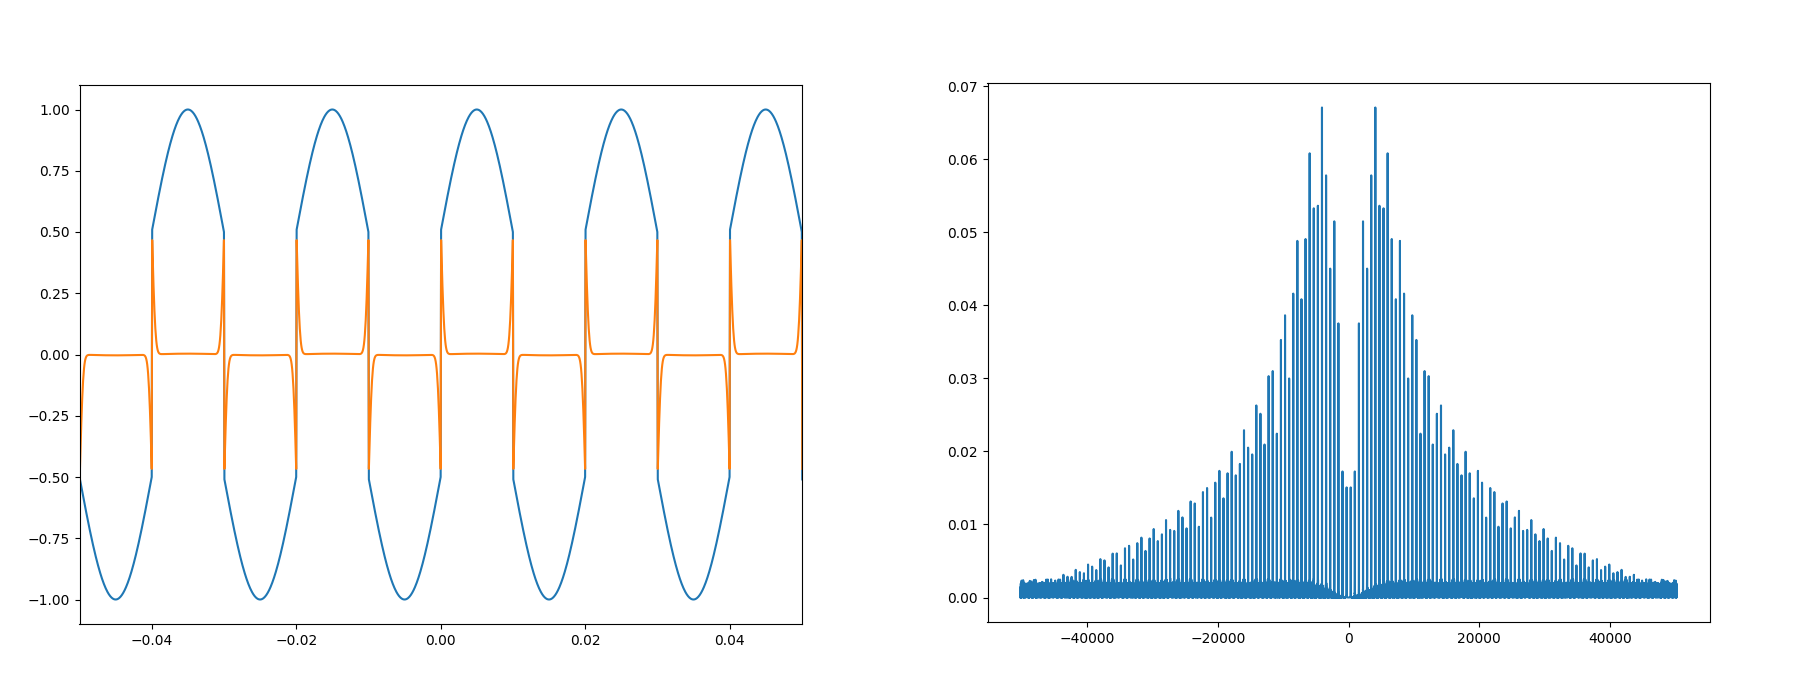
\includegraphics[scale=0.35\textscale]{r7graph03.png}
                                \caption{Representação gráfica do sinal filtrado pelo   sistema 5, a laranja (sobreposto sobre o sinal original, a azul) e espectro do sinal filtrado. De notar  a distinção nas variações lentas do sinal (inexistência total desta mesmas variações ), assim como a supressão da frequências mais baixas.}
                          \end{figure}
                        Assim como expectável as frequências mais baixas são suprimidas, resultando numa pior reprodução das variações lentas do sinal.
			\newpage
			\subsection{Questão R8}
			\paragraph{}
			Passando o sinal \textit{p} pelo sistema 6 e obtendo o módulo do espectro deste output:
			\begin{figure}[H]
                                    \centering
                                    \captionsetup{justification=centering}
                                    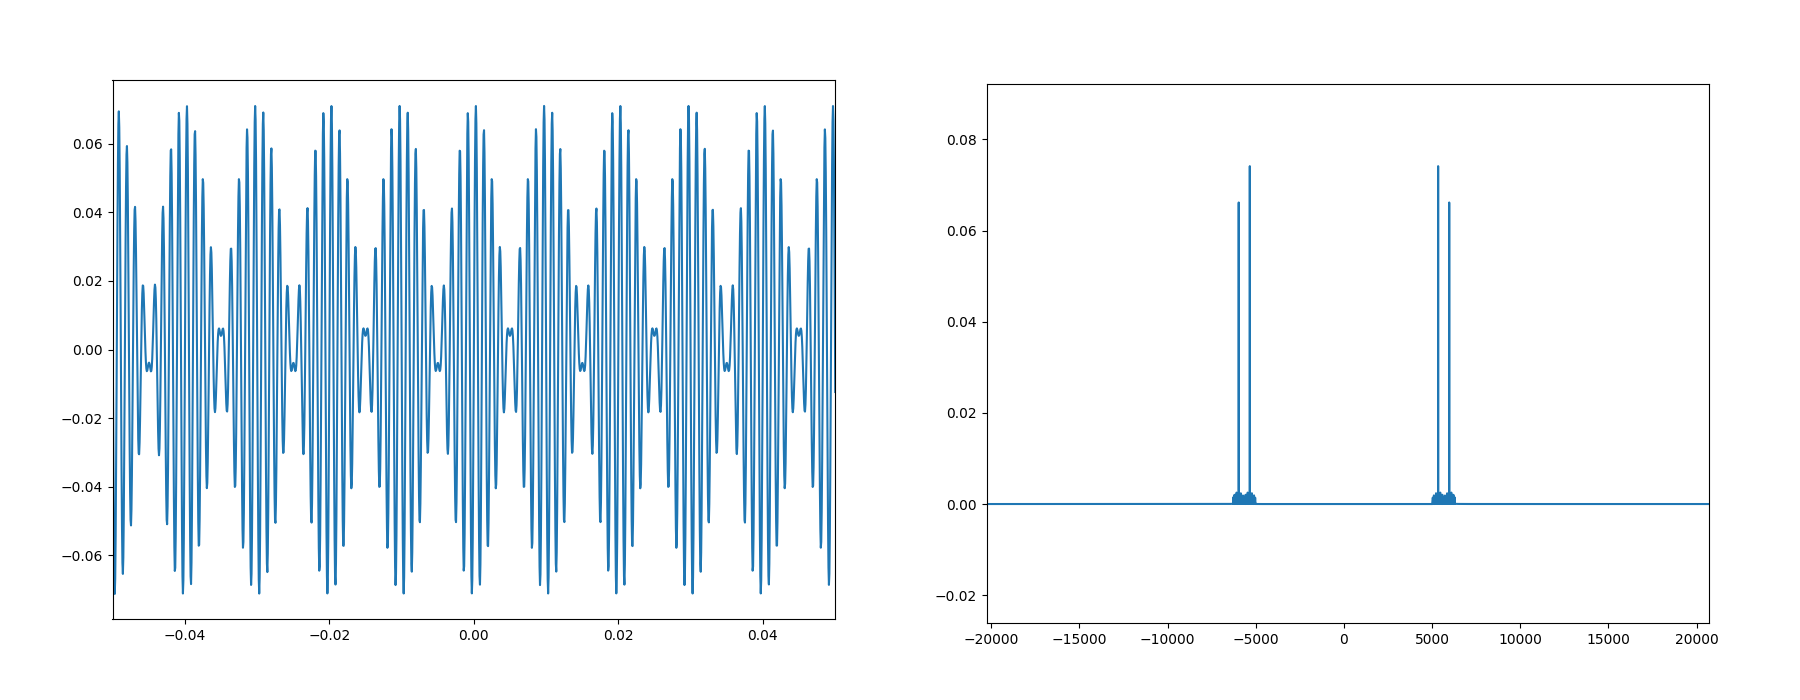
\includegraphics[scale=0.35\textscale]{r8graph03.png}
                                \caption{Representação gráfica do sinal filtrado pelo     sistema 6, e espectro do sinal filtrado. De notar os dois impulsos no espectro que limitam a banda passante com |$\omega _{min}$|=5430 rad/s e |$\omega_{max}$|=5969 rad/s}
                            \end{figure}
			Assim pela simples noção que $\frac{\omega}{2\pi} = f$ deduz-se que a banda passante se situa entre os 849.887Hz e os 949.996Hz.\\
			Adicionalmente compreende-se que o sinal obtido é a soma de dois senos, sin$_a$ e sin$_b$ com $\omega$$_a$ igual a 5340 rad/s e $\omega$$_b$ iguala 5969 rad/s. As amplitudes A$_a$ e A$_b$ podem ser deduzidas pela expressão Aa$_c$=A' com a$_c$=1.95 (amplitude de controlo obtida através de medição directa do espectro de sin(t)) e A' a amplitude de cada impulso do espectro de sistema6(\textit{p}) respectivamente A'$_a$=0.074 e A'$_b$=0.066. É então possível definir:
			\begin{center}
                                  \begin{math}
                                    sistema6(p)=0.038sin(5340t)+0.034sin(5969t)
                                  \end{math}
				  \mbox{}\\[0.5 cm]
				  Definição essa que pode ser interpretada num cenário de modulação pela identidade trigonométrica:\\
				  \begin{math}
                                      2sin(\theta)cos(\phi)=sin(\theta + \phi)+0.034sin(\teta - \phi)
                                    \end{math}
				  \mbox{}\\[0.5 cm] Obtendo-se assim:\\
				  \begin{math}
                                      sistema6(p)=0.072sin(5654.5t)cos(314.5t)                                    \end{math}
                        \mbox{}\\[0.5 cm]Utilizando a amplitude média dos senos de forma a ser resolúvel a identidade trigonométrica referida.
			\end{center}
			\newpage
			Obtêm-se então os outputs gráficos:
			\begin{figure}[H]
                                      \centering
                                      \captionsetup{justification=centering}
                                      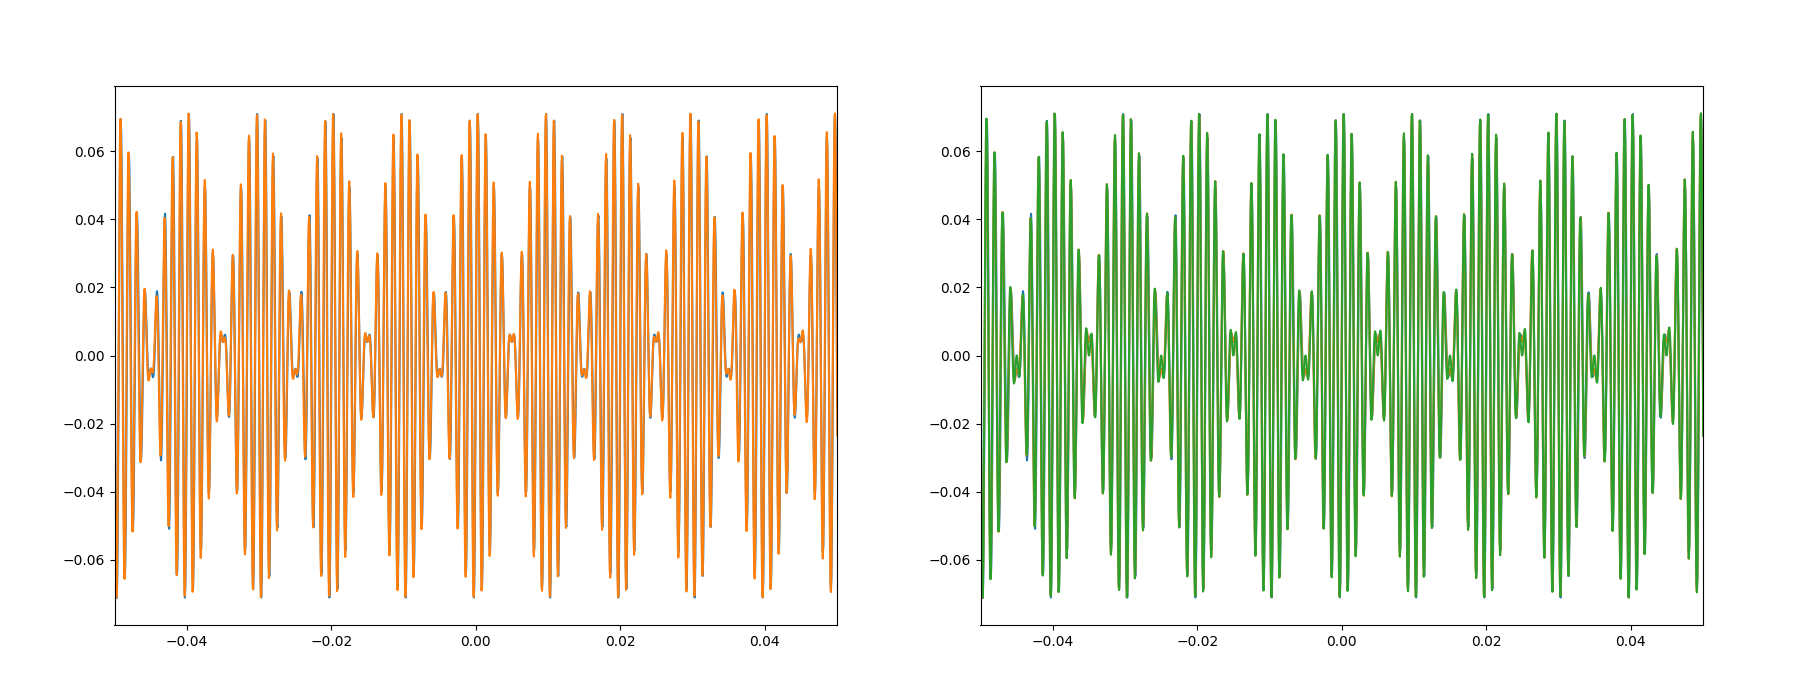
\includegraphics[scale=0.35\textscale]{r8graph04.png}
                               \caption{À esquerda: representação gráfica do sinal de saída formulado pela soma de senos (a laranja) sobre a representação gráfica inicial, de controlo (a azul). À direita: representação gráfica do sinal de saída formulado pela igualdade trigonométrica (a verde) sobre o a representação inicial, de controlo (a azul). De notar que em ambas as representações as distinções com o sinal de controlo são mínimas.}
                              \end{figure}
			Desta forma conclui-se que o output de sistema6(\textit{p}) é uma sinusoide uma vez que é o produto de duas sinusoides. Adicionalmente conclui-se que a frequência local do sinal de saída corresponde a 899.94 Hz e a de modulação a 50.05 Hz.

			\newpage
			\subsection{Questão R9}
                        \paragraph{Tomando como noção inicial a síntese do teorema da amostragem de Nyquist-Shannon:}
			\mbox{}\\
			\begin{center}
				É possível reter toda a informação de um sinal contínuo x$_c$$_1$ num sinal discreto x$_d$$_1$ se a frequência de amostragem \mathbb{f}$_a$ utilizada na síntese de x$_d$$_1$ pela amostragem de x$_c$$_1$ for igual ao superior ao dobro da frequência máxima presente no sinal x$_c$$_1$.
			\end{center}
			\mbox{}\\
			Amostrando o sinal x$_c$$_1$ com periodo de amostragem 0.01 segundos e reconstruindo o sinal com igual periodo obtém-se:
			\begin{figure}[H]
                                    \centering
                                    \captionsetup{justification=centering}
                                    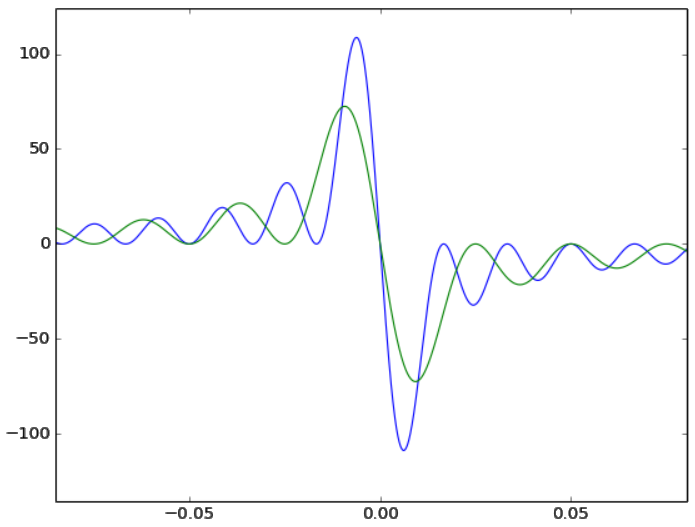
\includegraphics[scale=0.5\textscale]{r9graph01.png}
                                \caption{Representação gráfica do sinal y$_c$$_1$ reconstruído através da informação amostrada de x$_c$$_1$, a verde sobreposto sobre o sinal inicial, de controlo, a azul, x$_c$$_1$. De notar as distinções entre os dois gráficos, precipitando para a identificação de um caso de sub-amostragem.}
                            \end{figure}
			\newpage
			De forma a verificar a hipótese acima descrita sintetiza-se o módulo do espectro de x$_c$$_1$:
				\begin{figure}[H]
                                      \centering
                                      \captionsetup{justification=centering}
                                      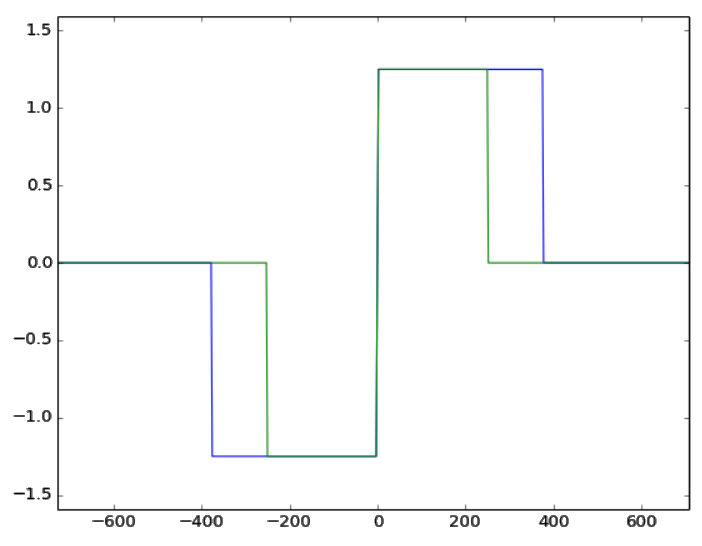
\includegraphics[scale=0.5\textscale]{r9graph03.png}
                                  \caption{Representação gráfica do espectro do sinal x$_c$$_1$ (a azul) subposto sobre o espectro do sinal y$_c$$_1$ (a verde). Por medição directa determina-se que $\omega$$_m$$_a$$_x$ presente no sinal x$_c$$_1$ é igual a 472.72 rad/s.}
                              \end{figure}
			A amostragem foi realizada com frequência de amostragem igual a 100 Hz e contudo verifica-se, por metódos anteriormente descritos, que a frequência máxima presente em x$_c$$_1$ é 75.23 Hz, ou seja de forma a reter toda a informação do sinal por amostragem, segundo o teorema da amostragem de Nyquist-Shannon, a frequência de amostragem teria que ser superior a 150.47 Hz ou seja periodo de amostragem igual ou inferior a 0.00646 segundos, condição essa que foi comprometida, originando na reconstrução do sinal a sobreposição de informação simétrica, originando o corte defrequências justificando a dintinção entre espectros.\\
			Assim conclui-se a presença de um caso de \textbf{sub-amostragem}.
	\newpage
		
		\bibliographystyle{plain}
		\nocite{ss}
		\bibliography{biblio}
	
\end{document}
